\synctex=1

%%%%
%%%% Multiagent Simulation and the MASON Library
%%%% Copyright 2010 by Sean Luke
%%%%
%%%% LaTeX Source
%%%% This source code, and embedded PDFs and sources (such as OmniGraffle Files)
%%%% Are distributed under the Academic Free License version 3.0
%%%% See the file "LICENSE" for more information
%%%%
%%%% When you build this source code, the resulting PDF file is licensed under the
%%%% Creative Commons Attribution-No Derivative Works 3.0 United States License
%%%% See the URL http://creativecommons.org/licenses/by-nd/3.0/us/   for more information
%%%%
%%%% If you have any questions, feel free to contact me at sean@cs.gmu.edu
%%%% Sean Luke

\documentclass[twoside,10pt]{book}
\usepackage{fullpage}
\usepackage{mathpazo}
\usepackage[noend]{algpseudocode}
\usepackage{amsmath}
\usepackage{latexsym}
\usepackage{graphicx}
\usepackage{wrapfig}
\usepackage{bm}
\usepackage{qtree}
\usepackage{array}
\usepackage{eurosym}
\usepackage{textcomp}
\usepackage{makeidx}
\usepackage{rotating}
\usepackage{multirow}
\usepackage{multicol}
\usepackage{microtype}
\usepackage{afterpage}
\usepackage{color}\definecolor{gray}{gray}{0.5}
\usepackage{alltt}
\usepackage{tabto}
\usepackage[font=footnotesize,labelsep=quad,labelfont=it]{caption}
\usepackage{todonotes}

\usepackage{listings}		% distributed 
\usepackage{xcolor}			% distributed

%%% Added in order to use hyperref -- this stuff has to appear before bibentry,x
%%% which has a conflict with regard to \bibitem.  See later in this file for more stuff that has
%%% to be added afterwards
  \makeatletter
  \let\saved@bibitem\@bibitem
  \makeatother

\usepackage{bibentry}
\usepackage[hyperfootnotes=false,linktocpage=true,linkbordercolor={0.5 0 0}]{hyperref}
%%% Note that to avoid a link being created from \pageref, just use \pageref*
%%% End hyperref stuff

\renewcommand\textfraction{0.0}
\renewcommand\topfraction{1.0}
\renewcommand\bottomfraction{1.0}


\newcommand\file[1]{\textsf{#1}}
\newcommand\variable[1]{\textsf{#1}}
%\newcommand\package[1]{\textsf{#1}}
\newcommand\package[1]{\index{Packages!{#1}}\textsf{#1}}
\newcommand\Package[1]{\index{Packages!{#1}|textbf}\textsf{#1}}
%\newcommand\class[1]{\textsf{#1}}
\newcommand\class[1]{\index{Classes!{#1}}\textsf{#1}}
\newcommand\Class[1]{\index{Classes!{#1}|textbf}\textsf{#1}}
\newcommand\method[1]{\hbox{\textsf{#1}}}
\newcommand\parameter[1]{\texttt{#1}}
\newcommand\character[1]{\texttt{"{#1}"}}
\newcommand\textstr[1]{\texttt{"{#1}"}}
\newcommand\code[1]{\textsf{#1}}

\newcommand\ignore[1]{}


\newcommand\sidebara[3]{\begin{wrapfigure}{r}[0in]{3.2in}%
\vspace{-1.1em}\hfill\framebox{\begin{minipage}{3in}\setlength\parindent{1.5em}\footnotesize{\noindent\textit{#1}

\vspace{0.5em}{\noindent #2}}
\end{minipage}}
\vspace{#3}
\end{wrapfigure}
}

\newcommand\sidebar[2]{\begin{wrapfigure}{r}[0in]{3.2in}%
\vspace{-1.1em}\hfill\framebox{\begin{minipage}{3in}\setlength\parindent{1.5em}\footnotesize{\noindent\textit{#1}

\vspace{0.5em}{\noindent #2}}
\end{minipage}}
\vspace{-0.5em}
\end{wrapfigure}
}



%%% Hack to allow more spacing before and after an hline
\newcommand\tstrut{\rule{0pt}{2.4ex}}
\newcommand\bstrut{\rule[-1.0ex]{0pt}{0pt}}

% Increase the numbering depth
\setcounter{secnumdepth}{3}
\setcounter{tocdepth}{6}


%%%% This code is used to create consistent lists of methods

% From TUGboat, Volume 24 (2003), No. 2 "Hints & Tricks"
\newcommand*{\xfill}[1][0pt]{%
	\cleaders
		\hbox to 1pt{\hss
			\raisebox{#1}{\rule{1.2pt}{0.4pt}}%
			\hss}\hfill}
			
\newenvironment{methods}[1]{
\vspace{1.0em}\noindent\textsf{\textbf{#1 Methods}}\quad \xfill[0.5ex]
\vspace{-0.25em}
\begin{description}
\small}
{\end{description}\hrule\vspace{1.5em}}

\newcommand{\mthd}[1]{\item[{\sf #1}]~\newline}


\newcommand\booktitle{DES documentation}
\newcommand\reference[1]{\vspace{0.5em}\hfill{\parbox{6in}{\raggedleft\noindent\textsf{#1}}}}

% Include subsubsection in the TOC
\setcounter{tocdepth}{3}

% Use with a %, like this:   \params{%
\newcommand\params[1]{\vbox{\begin{quote}\small\tt{\noindent{#1}}\end{quote}}}
\newcommand\script[1]{\params{#1}}
\newcommand\java[1]{\params{#1}}

% Allow poor horizontal spacing
\sloppy

% Allow a ragged bottom even in two-sided
\raggedbottom

% Command to push text to following page without the cutoff that occurs with clearpage
\newcommand\bump{\vspace{10in}}

% Command to push text to following line
\newcommand\hbump{\hspace{10in}}


% Define an existing word in text as an index item
\newcommand{\idx}[1]{\index{#1}#1}

% Define an existing word in text as an index item and make it bold
\newcommand{\df}[1]{\index{#1}\textbf{#1}}

% Provide a separate index item for a word in text and make it bold
\newcommand{\dfa}[2]{\index{#1}\textbf{#2}}

% Create algorithms and definitions
\newtheorem{algm}{Algorithm}
\newtheorem{defn}{Definition}

% Initial figures, pages, algorithms, and sections should be 0 :-)
\setcounter{figure}{-1}	% Mona is Figure 0
\setcounter{page}{-1}	% Start with Page 1 (the Front Page).  I'd like it to be Page 0 but it messes up twosided
\setcounter{algm}{-1}	% Start with Algorithm 0 (the Example Algorithm)
\setcounter{section}{-1}	% Start at Section 0 (the Introduction)

\thispagestyle{plain}
\thispagestyle{empty}

\newcommand\hsp[1]{{\rule{0pt}{0pt}\hspace{#1}}}
\newcommand\spc{{\rule{0pt}{0pt}~}}


%%%% Some stuff for Distributed

\lstdefinestyle{Bash}{
  language=bash,
  basicstyle=\small\sffamily,
  numbers=left,
  numberstyle=\tiny,
  numbersep=3pt,
  frame=tb,
  breaklines=true, 
  columns=fullflexible,
  backgroundcolor=\color{yellow!20},
  linewidth=0.9\linewidth,
  xleftmargin=0.1\linewidth
}

\definecolor{javared}{rgb}{0.6,0,0} % for strings
\definecolor{javagreen}{rgb}{0.25,0.5,0.35} % comments
\definecolor{javapurple}{rgb}{0.5,0,0.35} % keywords
\definecolor{javadocblue}{rgb}{0.25,0.35,0.75} % javadoc

\lstdefinestyle{CustomJava}{
    language=java,
    basicstyle=\ttfamily,
    keywordstyle=\color{javapurple}\bfseries,
    stringstyle=\color{javared},
    commentstyle=\color{javagreen},
    morecomment=[s][\color{javadocblue}]{/**}{*/},
    numbers=left,
    numberstyle=\tiny\color{black},
    stepnumber=2,
    numbersep=10pt,
    tabsize=2,
    showspaces=false,
    breaklines=true, 
    showstringspaces=false}





\makeindex


\begin{document}

\noindent\huge\bf \booktitle\\
\\
%{\large\rm A User Manual for the MASON Multiagent Simulation Toolkit}\\
\\
\Large\bf Sean Luke\\
{\large\rm 
Department of Computer Science\\
George Mason University}
\\
\\
\\
\large\rm {\bf Manual Version 1}\\
\large\rm November 2021\\

\clearpage



\normalsize
\cleardoublepage

\tableofcontents
\clearpage


\begin{figure}[t]
\centering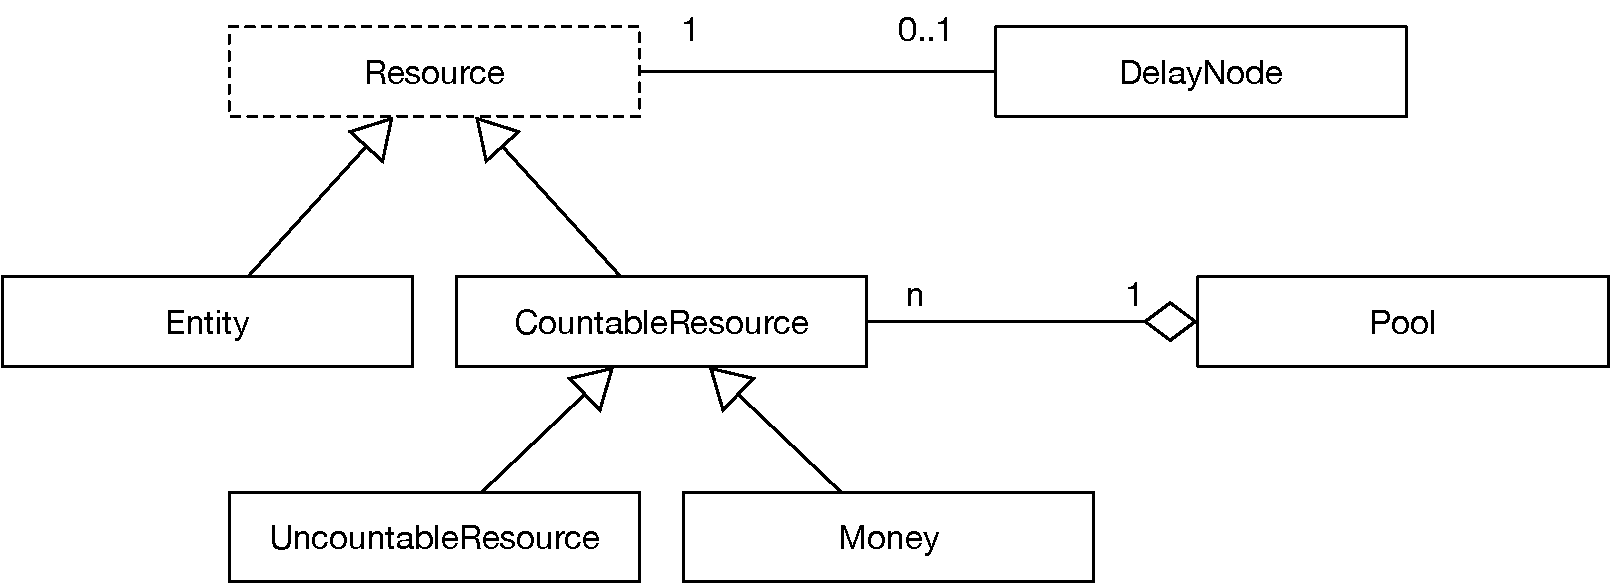
\includegraphics[width=3in]{Resources.pdf}
\end{figure}


\section{Resources}

Resources have two functions.  They either flow from Providers to Receivers, or they reside in a Pool shared by various Lock and Unlock objects.

\subsection{Resource}

Resource is the abstract superclass of resources.  All Resources have a {\bf unique type} (an int) shared by resources of that type, and a {\bf name} (String) which you can stipulate.  For example, all Electricity resources might have type 0, and all Gas resources might have type 1 and all Cars might have type 2 and all Dollars might have type 3.

\subsection{Entity}

An Entity is a Resource that cannot be subdivided.  For example: a Car might be an Entity.  But Water is not, as you can divide Water up into smaller amounts.  Entities can {\bf store} other resources inside them: that is, they can be {\bf composed} of them.  For example, a given Car might contain Wheels, and Engine, and some amount of Gasoline.  Different Cars are permitted to store different things.

\subsection{CountableResource}

A CountableResource is a Resource that has an {\bf amount} (an integer) and can be subdivided into CountableResources with smaller integer amounts.  For example: a Population might be divided into smaller subpopulations.  There is an atomic, smallest, non-divisible amount of CountableResources: 1.  You can also set the amount to 0.

\subsection{Money}

Money is a CountableResource with a cute printing function which prints it with a currency sign.  For example, a Dollar is Money, hence a CountableResource, where perhaps the smallest amount is the Cent (1).  Perhaps it should be renamed Cents.

\subsection{UncountableResource}

An UncountableResource is a CountableResource which can be subdivided infinitely and has real-valued amounts.  Thus while you can only have a CountableResource with values 0, 1, 2, 3, ...., an UncountableResource could be any positive amount, such as 0 or 2.34129 or 92.3 or Infinity.


\clearpage
\begin{figure}[t]
\centering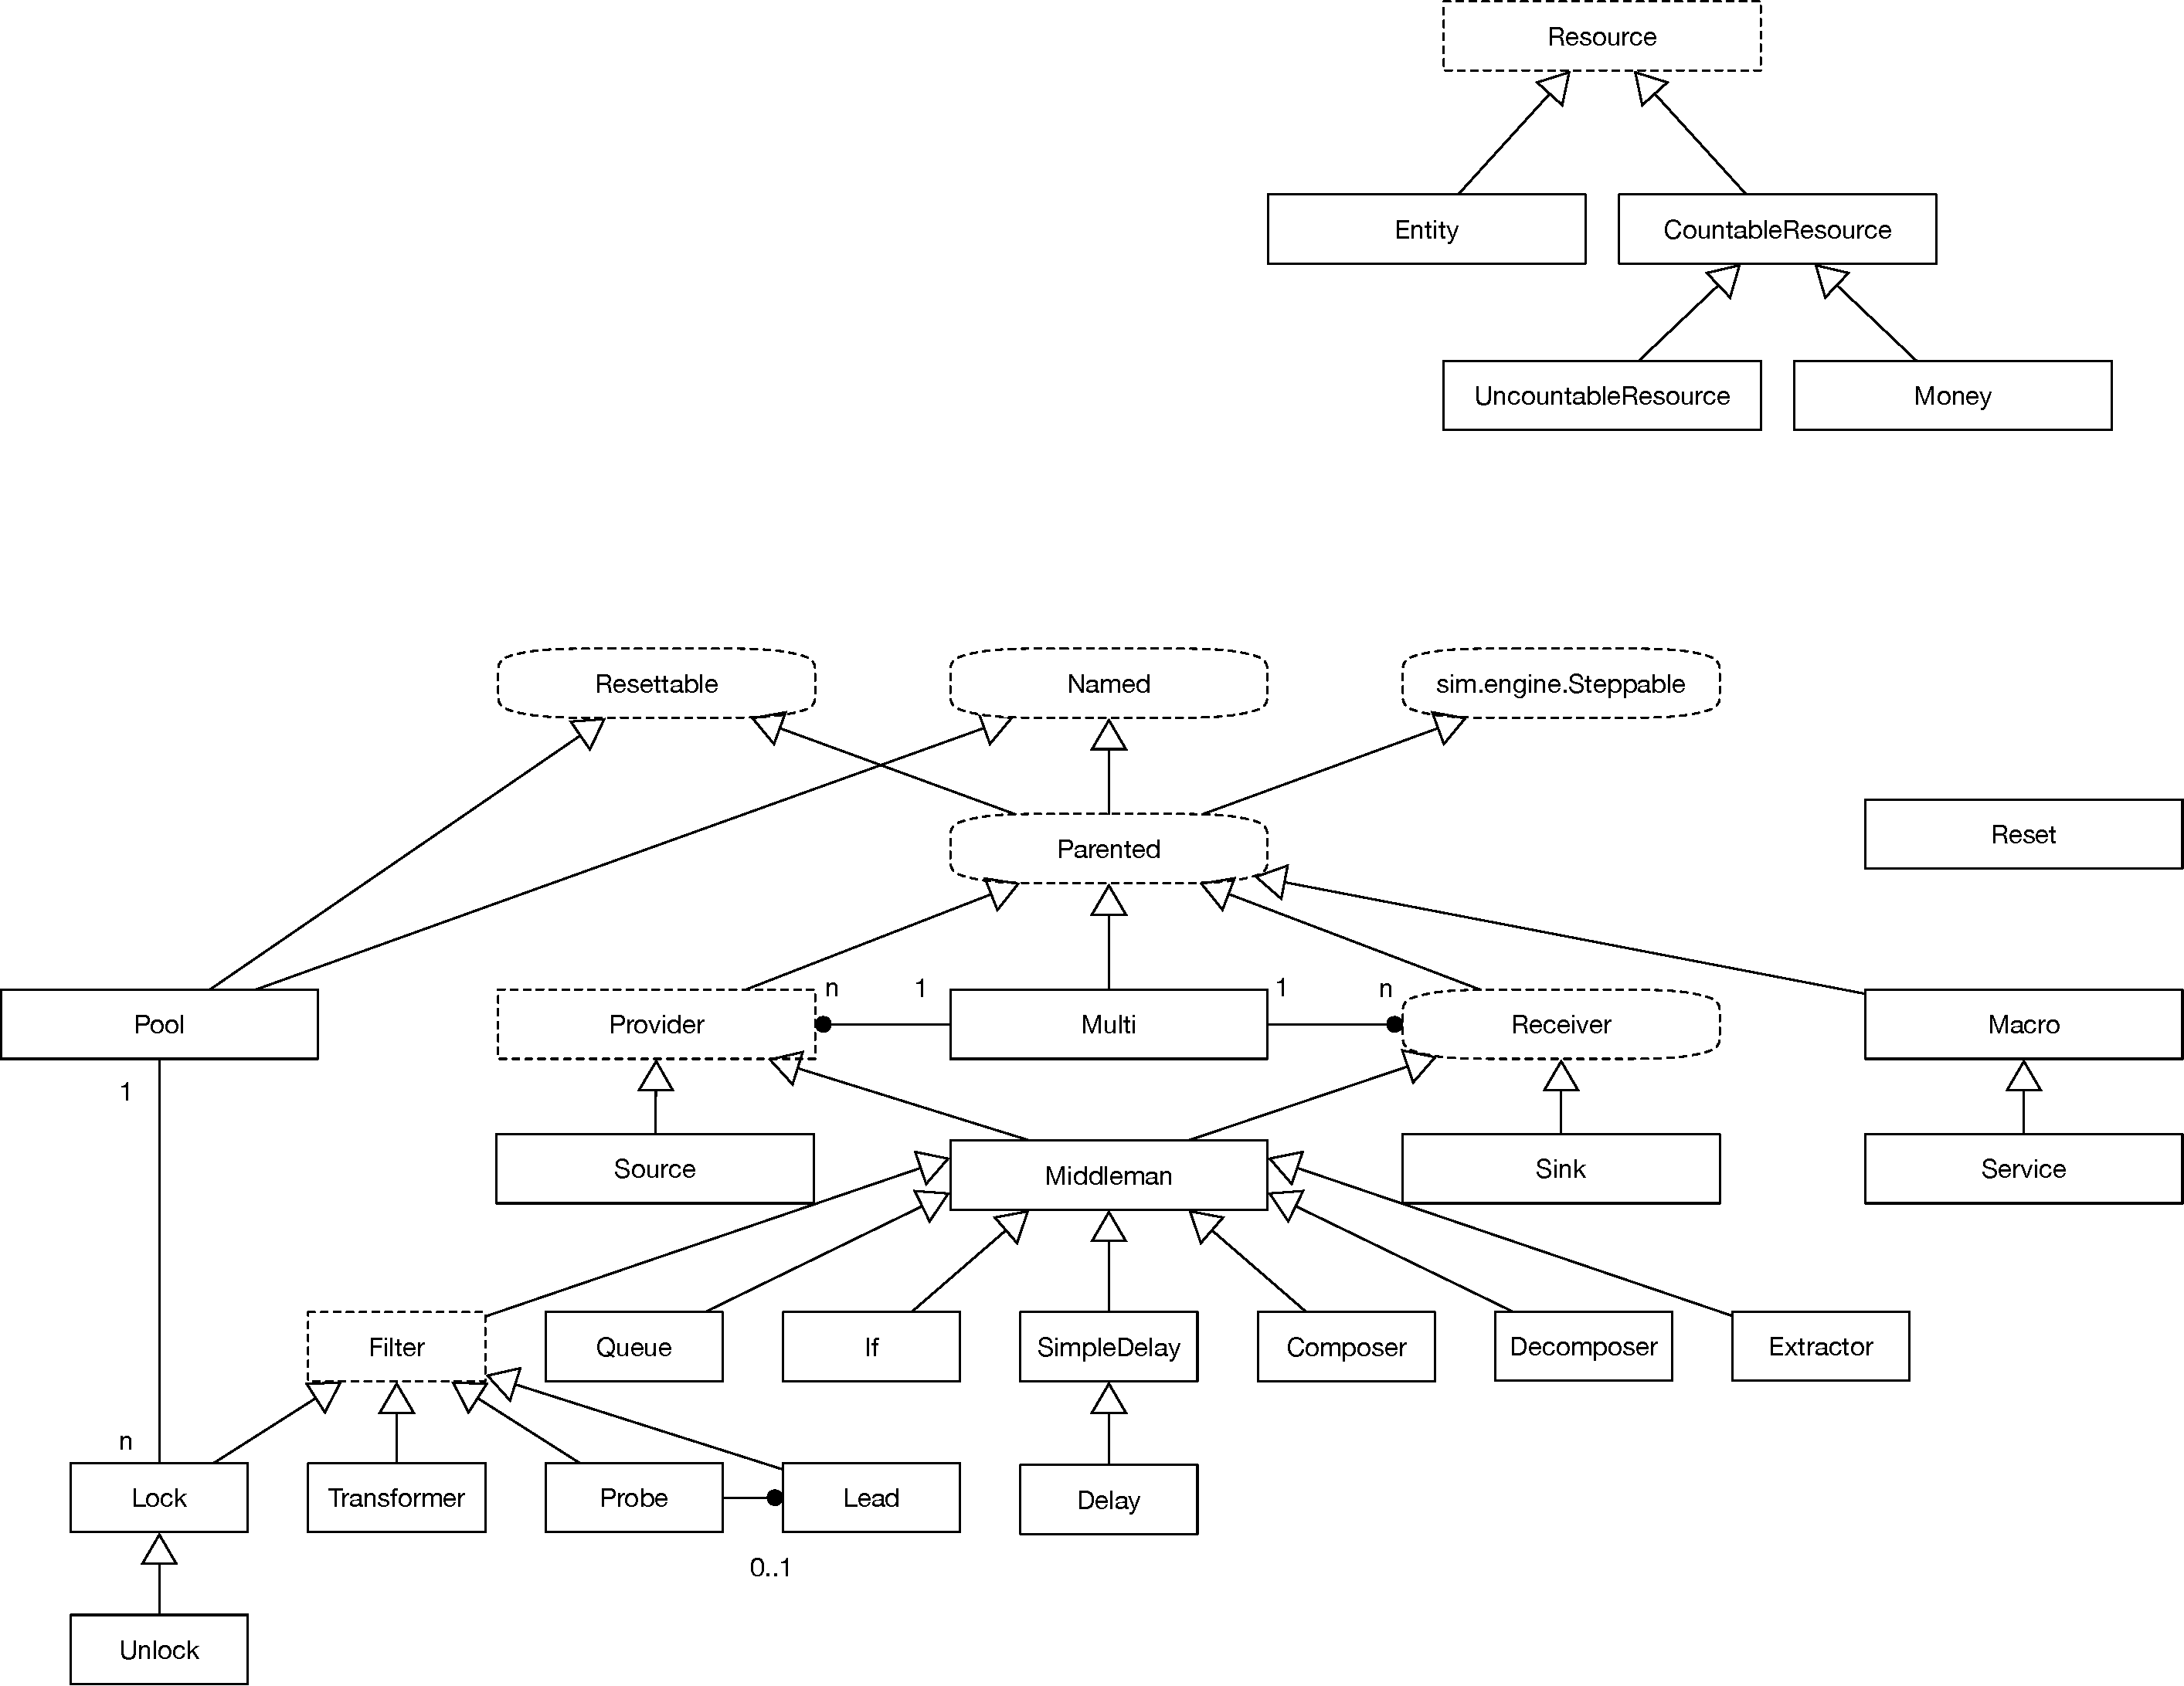
\includegraphics[width=6.5in]{Processes.pdf}
\end{figure}

\section{Processes}

Various Process objects can be {\bf Receivers} or {\bf Providers} or both, or compose these objects into groups called {\bf Macros}.  Most Process objects can be placed on MASON's schedule to be stepped when appropriate.

\subsection{sim.engine.Steppable}

An object which can be placed on MASON's schedule to be stepped in the future.

\subsection{Named}

A Steppable which also has a {\bf name} (a String).

\subsection{Resettable}

An object which can be {\bf reset} by a {\bf Reset} object.

\subsection{Receiver}

An object which can {\it receive} an offer from a Provider.  That is, the Provider will offer the Receiver some amount of Resource, asking it to {\bf accept} the offer.  Offers have minimum and maximum amounts that the Receiver may select from.  The receiver accepts some appropriate amount (between the min and max) of the Resource being offered by the Provider, or it refuses it.  A Receiver can also go to a Provider and {\bf ask} that the Provider make an offer to the Receiver.

\subsection{Sink}

A Receiver which accepts all offers (of the appropriate Resource type) and throws the resulting Resource away.  {\bf By default, this class's step() method does nothing, so there's no need to schedule it.}

\subsection{Provider}

An object which can make offers to one or more Receivers.  Receivers are {\bf registered} with the Provider.  When the Provider has a resource to offer, it will go to each of its Receivers according to some {\bf offer policy} and ask them to {\bf accept} offers of the Resource until it is depleted.  Providers can also be asked by a Receiver to make an offer to it.    Providers have a {\bf typical Resource type} of the resource that they offer.

\subsection{Source}

A Provider which generates Resources and offers it to downstream registered Receivers.  You can customize your Source however you want, but the default form works as follows.  Each time the Source is ready to {\bf produce} some Resource, the amount it produces is determined either by a {\bf distribution} or a {\bf deterministic amount}.  It then adds this Resource to a pile, and offers all the Resources currently in the pile to its receivers.  Sources have a maximum {\bf capacity} for their pile and will not generate more than this.  After making offers, the Source then uses {\it another} distribution or deterministic amount to determine the {\bf next time} it will generate Resources and make offers.  It schedules itself appropriately.

\subsection{Extractor}

Both a Receiver and a Source (sort of).  An Extractor is works like a Source, except that it ``builds'' its resources by extracting them from another Provider.  You could, for example, attach an Extractor to a Queue and every once i a while the Extractor would pull out of the Queue and offer resources to downstream Receivers.  Extractors ignore capacity.

\subsection{Queue}

Both a Receiver and Provider.  When a Queue receives a Resource, it adds it to a pile, then (usually) immediately offers this pile to its own receivers.  The Queue's pile has a maximum capacity.  If it cannot add to the pile, it will refuse the offer.

\subsection{SimpleDelay}

Both a Receiver and Provider.  When a SimpleDelay receives a Resource, it adds it to a linked list and, after a delay of some fixed amount of time, then offers the Resource to downstream receivers.  If the receivers do not accept, then the Resource is discarded.  The SimpleDelay has a maximum capacity of items it may store which are presently delayed.

\subsection{Delay}

A subclass of SimpleDelay.  This is just like a SimpleDelay, except that the delay time for each object received can be {\it different}, so some Resources can move through the Delay faster than others.  Thus the SimpleDelay is implemented using a heap rather than a linked list.

\subsection{Composer}

Both a Receiver and Provider.  Upon receiving a Resource, it adds it to a collection of Resources. These Resources can be of different types.  When it has all the necessary amounts of Resources for each type, it gathers them together and produces a Composed Entity holding these Resources, then offers the Entity to downstream receivers. If they do not accept, then the Entity is discarded.  The Composer has both minimum and maximum (capacity) amounts for each of the Resources needed to compose into the Entity.

\subsection{Decomposer}

Both a Receiver and Provider.  Upon receiving a Composed Entity, it decomposes it and offers each of its Resources to various downstream receivers, one registered for each Resource type. If they do not accept, then that Resource is discarded.  {\bf By default, this class's step() method does nothing, so there's no need to schedule it.}



\section{Filters}

Filters are just Processes which accept offers and immediately turn around and offer them to a single downstream Receiver.  Filters are both Providers and Receivers, and never respond to requests to make offers.

\subsection{Filter}

The abstract superclass of Filters, which simply gathers together variables and methods common to them.

\subsection{Transformer}

Upon receiving a Resource, Transformer {\bf transforms} the Resource into a different one according to a certain rule, then immediately offers it to downstream receivers.  If they do not accept, then the Resource is discarded.  {\bf By default, this class's step() method does nothing, so there's no need to schedule it.}

\subsection{Lock}

Upon receiving a Resource, Lock attempts to {\bf allocate} some amount of {\it a different} Resource from a {\bf Pool}.  If successful, it then offers the original Resource to downstream receivers. If they do not accept, then that Resource is discarded.  {\bf By default, this class's step() method does nothing, so there's no need to schedule it.}

\subsection{Unlock}

A subclass of Lock, but only for convenience's sake.  Upon receiving a Resource, it {\bf provides} some amount of {\it a different} Resource to a {\bf Pool}.  Regardless of whether the Pool accepts this generosity, Unlock then offers the original Resource to downstream receivers. If they do not accept, then that Resource is discarded.  {\bf By default, this class's step() method does nothing, so there's no need to schedule it.}

\subsection{Probe}

An object which gathers statistics on the resources which pass through it.  A Probe can also be used in conjunction with a {\bf Lead}.

\subsection{Lead}

An object detached from Probe with can be used in combination with it to determine the amount of resources in a DES subgraph between them.

\subsection{If}

A Filter which receives and incoming offer, then chooses only one of several possible Receivers to hand the offer to.  This choice is specified in a method defined by the modeler.

\section{Process Utilities}

\subsection{Pool}

A shared pool of a Resources which may be allocated or provided by Lock and Unlock objects.  {\bf By default, this class's step() method does nothing, so there's no need to schedule it.}

\subsection{Macro}

An object which can store a {\bf subgraph} of the DES graph.  This subgraph consists of some {\bf Receivers}, some {\bf Providers}, and some {\bf in-between Processes}.  When stepped, the Macro steps all of its stored objects in order.  You can access the Receivers and Providers to make offers or register stuff as you see fit.

\subsection{Service}

A simple example of a common Macro consisting of a Lock, then a SimpleDelay, then an Unlock.

\subsection{Reset}

Collects a bunch of {\bf Resettable} objects and allows you to easily {\bf reset} all of them.  This way you can create your DES graph in the model's constructor, then reset it each time you {\bf start()} the model, by just calling {\bf reset()} on your Reset in the body of the start() method.



%\cleardoublepage
%\footnotesize
%\addcontentsline{toc}{chapter}{Index}
%\printindex

\end{document}














